The radius of the circle below is 4 meters. If the area of the shaded region is $6\pi$, what does \textit{a} equal in degrees?

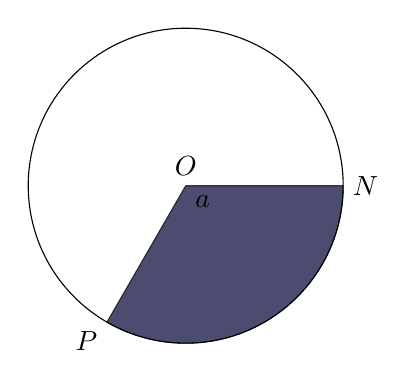
\begin{tikzpicture} 
\draw(0,0)node[anchor=south]{$O$}circle(2); 
\fill[draw=black,fill=blue!20!black,opacity=0.7](0,0)--(2,0)arc(0:-120:2)--(0,0); 
\draw(2,0)node[anchor=west]{$N$}(-120:2)node[anchor=north east]{$P$}; 
\draw(0,0)node[anchor=north west]{$a\degree$}; 
\end{tikzpicture} 

\ifsat
	\begin{enumerate}[label=\Alph*)]
		\item  $60\degree$ 
		\item  $80\degree$ 
		\item  $115\degree$ 
		\item  $135\degree$ %
	\end{enumerate}
\else
\fi

\ifacteven
	\begin{enumerate}[label=\textbf{\Alph*.},itemsep=\fill,align=left]
		\setcounter{enumii}{5}
		\item   $.375$
		\item  $60\degree$ 
		\item  $80\degree$
		\addtocounter{enumii}{1}
		\item  $115\degree$ 
		\item  $135\degree$ %
	\end{enumerate}
\else
\fi

\ifactodd
	\begin{enumerate}[label=\textbf{\Alph*.},itemsep=\fill,align=left]
		\item   $.375$
		\item  $60\degree$ 
		\item  $80\degree$ 
		\item  $115\degree$ 
		\item  $135\degree$ %
	\end{enumerate}
\else
\fi

\ifgridin
  $135\degree$ %

\else
\fi

